\documentclass[mathserif]{beamer}
\usepackage{appendixnumberbeamer}
\usepackage[nofirafonts]{beamerthemefocus}
\usepackage{amsmath}
\usepackage{graphicx}
\usepackage{natbib}
\usepackage{floatrow}
\usepackage{booktabs}
\usepackage{multirow}

\usepackage{xeCJK}
\setCJKmainfont{Iansui094-Regular}

\title{檢視中國債務陷阱\\Examining the Chinese Debt-Trap Diplomacy}
\author{陳家威\\{\small R10323045}}
\date{112年7月12日}

\begin{document}

    \begin{frame}

        \maketitle

    \end{frame}

    \section{Debt Trap}
    \begin{frame}
        \frametitle{Debt-trap Diplomacy}

        \begin{block}
            {Debt-trap Diplomacy}
            China extends excessive loans to countries and places a debt burden upon them in exchange
            for political or economic concessions.
        \end{block}
    \end{frame}

    \begin{frame}
        \frametitle{Debt to China}
            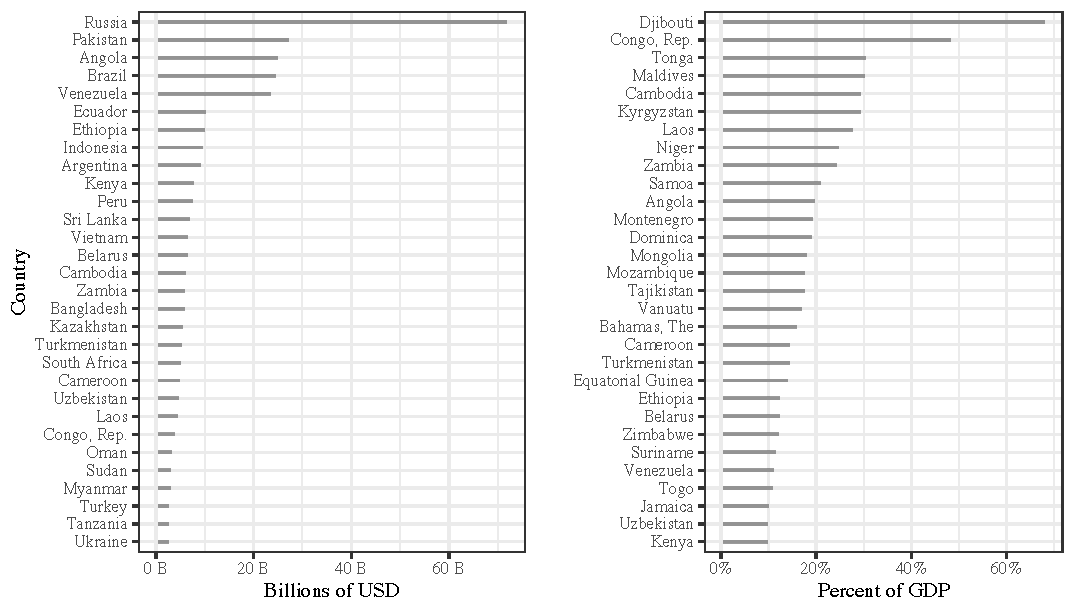
\includegraphics[width = \textwidth]{fig/debt-level-by-country.pdf}
    \end{frame}

    \begin{frame}
        \frametitle{Sri Lanka Project List}
        Hambantota Port
        \begin{itemize}
            \item Initiated: 2007
            \item 2008: Phase I, \$307 million from Chinese Exim Bank, 6\% rate
            \item 2012: Phase II, \$304 million
            \item 2017: 99-year lease, 70\% sale to China Merchant Port
        \end{itemize}
        \vfill
        Mattala Rajapaksa International Airport
        \begin{itemize}
            \item 2009: \$181 million from Chinese Exim Bank, 2\% rate
            \item 2013: Open
            \item 2014: 21,000 passengers only
            \item ``The world's emptiest airport'
        \end{itemize}
        \vfill
        Road Projects
        \begin{itemize}
            \item 2009: \$1.14 billion Colombo-Katunayake Expressway (CKE)
            \item 2010\&2011: 1.51\%
            \item 2014: \$1.99 on road construction and improvement
        \end{itemize}
    \end{frame}

    \begin{frame}
        \frametitle{Pakistan Project List}
        Power Project 2016
        \begin{itemize}
            \item \$2.7 billion on the Gwadar-Nawabshah LNG terminal and pipeline project;
            \item \$1.26 billion on the Karot Hydropower Project;
            \item \$1.28 billion on the Matiari to Lahore Transmission Line;
            \item \$1.55 billion on the Pakistan Port Qasim Power Project; and \$0.75 billion on the Qasim Datang Power Station \citep*{Horn-Reinhart-Trebesch-21}.
        \end{itemize}
        \vfill
        Power Project 2017
        \begin{itemize}
            \item \$1.35 billion for Suki Kinari Hydropower Project
            \item \$1.5 billion on the Hubco Coal Power Plant Project
        \end{itemize}
        \vfill
        Gwadar Port
        \begin{itemize}
            \item 2015: 43-year lease to China Overseas Port Holding Company
            \item Develope Special Economic Zone (SEZ)
        \end{itemize}
    \end{frame}

    \section{Model}
    \begin{frame}
        \frametitle{Model Setting}

        \begin{itemize}
            \item Decentralized version of Eaton-Gersovitz model
            \item Tradable vs Nontradable goods
            \item Household, Firm, Government, Foreign lender
        \end{itemize}

    \end{frame}

    \begin{frame}
        \frametitle{Household}
        \begin{itemize}
            \item Maximize
                \begin{equation}
                    E_0 \sum_{t=0}^\infty \beta^t U(c_t)
                \end{equation}
            \item Utility function
                \begin{equation}
                    U(c_t) = \frac{c_t^{1-\sigma} - 1}{1 - \sigma}
                \end{equation}
            \item Aggregation function for consumption
                \begin{equation}
                    \label{eq:aggregator-function}
                    c_t = A(c^T_t, c^N_t) =
                        \left[ a \left( c^T_t \right)^{1- \frac{1}{\xi}} +
                            (1 - a) \left( c^N_t \right)^{1- \frac{1}{\xi}}
                        \right]^{\frac{1}{1 - \frac{1}{\xi}}}
                \end{equation}
            \item Budget constraint
                \begin{equation}
                    \label{eq:bc}
                    P^T_t c^T_t + P^N_t c^N_t + P^T_t d_t =
                    P^T_t \tilde{y}^T_t + W_t h_t + (1- \tau^d_t)P^T_t q^d_t d_{t+1} + F_t + \Phi_t
                \end{equation}
            \item Working hours
                \begin{equation}
                    \label{eq:h-constraint}
                    h_t \le \bar{h}
                \end{equation}
        \end{itemize}
    \end{frame}

    \begin{frame}
        \frametitle{HH F.O.C}
        Notation:
$p_t \equiv \frac{P^N_t}{P^T_t}$, $w_t = \frac{W_t}{P^T_t}$, $f_t = \frac{F_t}{P^T_t}$, and $\phi_t = \frac{\Phi_t}{P^T_t}$
            \begin{subequations}
                \begin{align}
                    p_t &= \frac{A_2(c_t^T, c_t^N)}{A_1(c_t^t, c_t^N)} \label{eq:FOC-HH-1} \\
                    \lambda_t &= U'(c_t)A_1(c_t^T, c_t^N)\\
                    (1-\tau_t^d)q_t^d \lambda_t &= \beta E_t \lambda_{t+1}
                \end{align}
            \end{subequations}
    \end{frame}

    \begin{frame}
        \frametitle{Firms}
            \begin{itemize}
                \item Technology
                    \begin{equation}
                        \label{eq:production}
                        y^N_t = F(h_t)
                    \end{equation}
                \item Profit
                    \begin{equation}
                        \label{eq:profit}
                        \Phi_t(h_t) = P^N_t F(h_t) - W_t h_t
                    \end{equation}
                \item F.O.C
                    \begin{equation}
                        \label{eq:firm-FOC}
                        p_t F'(h_t) = w_t
                    \end{equation}
            \end{itemize}
    \end{frame}

    \begin{frame}
        \frametitle{Downward Wage Rigidity}

        \begin{equation}
            W_t \ge \gamma W_{t-1}, \qquad \gamma > 0
        \end{equation}
        This implies that the growth rate
        $\frac{W_{t} - W_{t-1}}{W_{t-1}} \ge \gamma - 1$

        \vfill
        Slackness condition

        \begin{equation}
            \label{eq:wage-rigid}
            (\bar{h} - h_t)(W_t - \gamma W_{t-1}) = 0
        \end{equation}
    \end{frame}

    \begin{frame}
        \frametitle{Government}

        Government decides to default of not for the economy
        \begin{itemize}
            \item If repay $(I=1)$: able to lend in $t+1$, or $d_{t+1} > 0$
            \item If default $(I=0)$: excluded from international credit market, $d_{t+1} = 0$
        \end{itemize}
        Written as slackness condition
        \begin{equation}
            \label{eq:gov-next-debt}
            (1 - I_t)d_{t+1} = 0
        \end{equation}
        \vfill
        Government returns tax to household via lump-sum transfer

        \begin{equation}
            \label{eq:gov-budget}
            f_t = \tau_t^d q_t^d d_{t+1} + (1-I_t)d_t
        \end{equation}
        \begin{itemize}
            \item If repay $(I=1)$: gives back $\tau_t^d q_t^d d_{t+1}$
            \item If default $(I=0)$: further distribute current debt $d_t$
        \end{itemize}

    \end{frame}

    \begin{frame}
        \frametitle{Foreign lender}

        \begin{itemize}
            \item Risk neutral
            \item If country in good standing, offer price $q_t$ for debt that returns 1 unit of $d_{t+1} \rightarrow$ return on debt $=\frac{1}{q_t}$
            \item take future default events into evaluation
                \begin{equation}
                    \label{eq:lender}
                    \frac{\Pr(I_{t+1}=1 \mid I_{t}=1)}{q_t} = 1 + r^*
                \end{equation}
            \item Slackness condition
                \begin{equation*}
                    I_t \left[ q_t - \frac{E_t I_{t+1}}{1+r^*} \right] = 0
                \end{equation*}

        \end{itemize}

    \end{frame}

    \begin{frame}[allowframebreaks]
        \frametitle{Competitive Equilibrium}
        Output
        \begin{itemize}
            \item Nontradable goods
            \begin{equation}
                c^N_t = y^N_t
            \end{equation}
            \item tradable goods
                \begin{equation}
                    \label{eq:ar1-output}
                    \ln(y_t^T) = \rho \ln(y^T_{t-1}) + \mu_t
                \end{equation}
            \item Endowment loss under bad standing $(I_t= 0)$
                \begin{equation}
                    \label{eq:ytt}
                    \tilde{y}^T_t =
                        \begin{cases}
                        y^T_t  - L(y^T_t) & \text{if } I_t = 0 \\
                        y^T_t & \text{otherwise.}
                        \end{cases}
                \end{equation}
            \item $L(y^T_t) = \max \{0, \delta_1 y^T_t + \delta_2 (y^T_t)^2\}$
                \framebreak
            \item price demand = price supply during good standing
                \begin{equation}
                    \label{eq:qq}
                    I_t(q^d_t - q_t) = 0
                \end{equation}
            \item combine above with budget constraint
                \begin{equation}
                    \label{eq:market-clearing}
                    c^T_t = y^T_t - (1 - I_t)L(y^T_t) + I_t(q_t d_{t+1} - d_t)
                \end{equation}
                \framebreak
            \item law of one price $P^T_t = P^{T*}_t \mathcal{E}_t$
            \item normalize foreign currency price to 1L $P^T_t = \mathcal{E}_t$
            \item devaluation rate
                \begin{equation}
                    \label{eq:devaluation-rate}
                    \epsilon_t \equiv \frac{\mathcal{E}_t}{\mathcal{E}_{t-1}} = \frac{P^T_t}{P^T_{t-1}}.
                \end{equation}
            \end{itemize}
    \end{frame}

    \begin{frame}[allowframebreaks]
        \frametitle{CE}
        $\left\{ c^T_t, h_t, w_t, d_{t+1}, \lambda_t, q_t, q^d_t \right\}$ satisfying:
        \framebreak
        {\small
            \begin{align}
    c^T_t &= y^T_t - (1 - I_t)L(y^T_t) + I_t(q_t d_{t+1} - d_t), \\
    (1 - I_t)d_{t+1} &= 0, \\
    \lambda_t &= U'(A(c^T_t, F(h_t)))A_1(c_t^T, c_t^N),\\
    (1-\tau_t^d)q_t^d \lambda_t &= \beta E_t \lambda_{t+1}, \\
    I_t(q^d_t - q_t) &= 0, \\
    \frac{A_2(c_t^T, F(h_t))}{A_1(c_t^t, F(h_t))} &= \frac{w_t}{F'(h_t)} , \\
   w_t &\ge \gamma\frac{w_{t-1}}{\epsilon_t},\\
   h_t &\le \bar{h},\\
   \left( h_t - \bar{h} \right) \left( w_t - \gamma\frac{w_{t-1}}{\epsilon_t}\right) &= 0, \\
    I_t \left[ q_t - \frac{E_t I_{t+1}}{1+r^*} \right] &= 0,
\end{align}
        }
        \framebreak
        given processes $\left\{ y^T_t, \epsilon_t, \tau^d_t, I_t \right\}$ and initial conditions $w_{-1}$ and $d_0$.
    \end{frame}

    \begin{frame}
        \frametitle{Default decision}
               \small
            \begin{equation}
                \label{eq:vc}
                \begin{aligned}
                    v^c(y^T_t, d_t) = \max_{\left\{ c^T_t, h_t, d_{t+1} \right\}} \quad
                    &\left\{
                        U\left(
                            A\left(c^T_t, F(h_t)\right)
                        \right)
                        + \beta E_t
                        v^g \left(
                            y^T_{t+1}, d_{t+1}
                        \right)
                    \right\}\\
                    \text{s.t} \quad& c^T_t + d_t = y^T_t + q(y^T_t, d_{t+1}) d_{t+1} \\
                                & h_t \le \bar{h}.
                \end{aligned}
            \end{equation}
            \begin{equation}
                \label{eq:vb}
                \begin{split}
                    v^b(y^T_t) = \max_{\left\{ h_t \right\}} \quad
                    &\Bigg\{
                        U\left(
                            A\left( y^T_t - L(y^T_t), F(h_t)\right)
                        \right)
                        + \\
                        & \beta E_t \left[
                            \theta v^g \left(
                                y^T_{t+1}, 0
                            \right)
                            + (1-\theta) v^b \left(
                                y^{T}_{t+1}
                            \right)
                        \right]
                    \Bigg\}\\
                    \text{s.t} \quad& h_t \le \bar{h}.
                \end{split}
            \end{equation}
            \begin{equation}
                \label{eq:vg}
                v^g(y^T_t, d_t) = \max\left\{
                    v^c(y^T_t, d_t) ,
                    v^b(y^T_t)
                \right\}.
            \end{equation}
    \end{frame}

    \begin{frame}
        \frametitle{Default set}
        \begin{itemize}
            \item Given a debt level $d_t$, the output under which default is optimal
            \begin{equation}
                \label{eq:default-set}
                D(d_t) = \left\{
                    y^T_t : v^b(y^T_t) > v^c(y^T_t, d_t)
                    \right\}.
                \end{equation}
            \end{itemize}
    \end{frame}
    \begin{frame}
        \frametitle{Plotting the default set}
        \begin{itemize}
            \item Gray: Non-default set
            \item White: Default set
        \end{itemize}
        \centering
        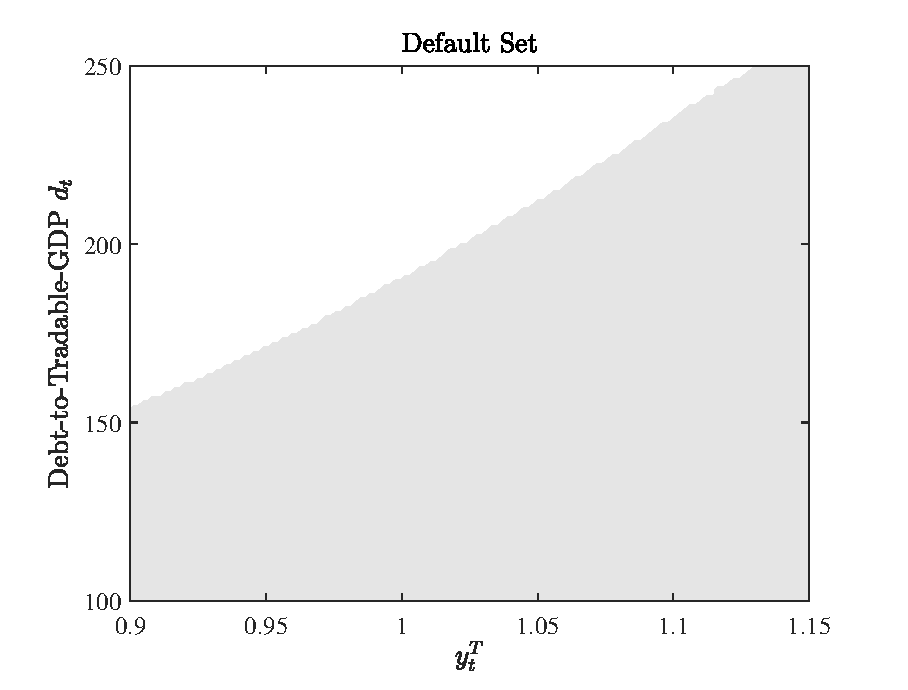
\includegraphics[height = 0.7\textheight]{fig/default_set_sri_trad_hp.eps}

    \end{frame}

    \begin{frame}
        \frametitle{Price of Debt}
        \begin{itemize}
            \item $\Pr(I_{t+1}=1 \mid I_{t}=1)$ is probability that next period output falls into default set
            \begin{equation}
                q(y^T_t, d_{t+1}) =
                \frac{1 - \Pr\left\{ y^T_{t+1} \in D(d_{t+1}) \mid y^T_t \right\}}{1 + r^*}
            \end{equation}
            \item Since $y^T_t$ is AR(1), output today is enough information about tomorrow $\rightarrow$ function of $y^T_t$
        \end{itemize}
    \end{frame}

    \begin{frame}
        \frametitle{Optimal Devaluation Rate}
        \begin{itemize}
            \item Optimal labor supply: $h_t = \bar{h}$ or full employment
            \item To ensure full employment, wage must be
                \begin{equation}
                    w_t = w^f(c^T_t) \equiv \frac{A_2(c^T_t, F(\bar{h}))}{A_1(c^T_t, F(\bar{h}))} F'(\bar{h})
                \end{equation}
            \item Because downward rigidity
                \begin{equation*}
                    \gamma \le \frac{W_t}{W_{t-1}} = \frac{w_t}{w_{t-1}} \frac{P^T_t}{P^T_{t-1}} = \epsilon \frac{w_t}{w_{t-1}}
                \end{equation*}
            \item Optimal devaluation rate is any $\epsilon_t$ such that
                \begin{equation}
                    \epsilon_t \ge \gamma \frac{w_{t-1}}{w^f(c^T_t)}
                \end{equation}
        \end{itemize}
    \end{frame}

    \section{Calibration}
    \begin{frame}
        \frametitle{Parameters needed to be calibrated}
        \begin{tabular}[t]{r l}
            Param. & Description \\
            \hline\\
            $\rho$     & Autocorrelation of output\\
            $\sigma_u$ & Standard deviation of output\\
            $r^*$      & Risk-free rate\\
            $\theta$   & Probability of reentry\\
            $\alpha$   & Labor share in nontradable goods sector\\
            $a$        & Share of tradable consumption\\
            $\xi$      & Intratemporal elasticity of substitution of consumptin\\
            $\sigma$   & 1/(intertemperal elasticity of substitution of consumption)\\
            $\gamma$   & Downward wage rigidity\\
            $\beta$    & Discount factor\\
            $\delta_1$ & Coefficient of the linear term in loss function\\
            $\delta_2$ & Coefficient of the quadratic term in loss function\\

            \end{tabular}
    \end{frame}

   \begin{frame}
    \frametitle{General procedure}
    \begin{itemize}
        \item $\rho, \sigma_u$:  Per capita tradable GDP $\rightarrow$ HP-filter $\rightarrow$ cyclical component $\rightarrow$ AR(1) estimation $\rightarrow \hat{\rho}, \hat{\sigma}_u$
        \begin{itemize}
            \item Since model period is quarter, data period is year
            \item $\rho = 1 - \frac{1 - \hat{\rho}}{4}$, $\sigma_u = \frac{\hat{\sigma}_u}{\sqrt{4}}$
        \end{itemize}
        \item $r^*$: US 3-month T-bill $\approx 4\%$ per year
        \item $\theta$: 1 / average years till reentry
        \item $\alpha$: Follow calibration of literature
        \item $a$: mean of tradable-to-GDP ratio over 1980 to 2021
        \item $\sigma, \xi$: Follow literature, set as (2, 0.5)
        \item $\beta, \delta_1, \delta_2$: match three equilibrium moment
        \begin{itemize}
            \item Quarterly unsecured debt-to-tradable-GDP ratio
            \item Default frequency per century
            \item Average output loss in bad standings
        \end{itemize}
    \end{itemize}
   \end{frame}

   \begin{frame}[allowframebreaks]
    \frametitle{Output process}
        \begin{itemize}
            \item HP-filter with $\lambda = 100$ since annual data
            \item Also tried log-quadratic detrend
            \item Tradable = agriculture + forestry + fishing + industry
        \end{itemize}

        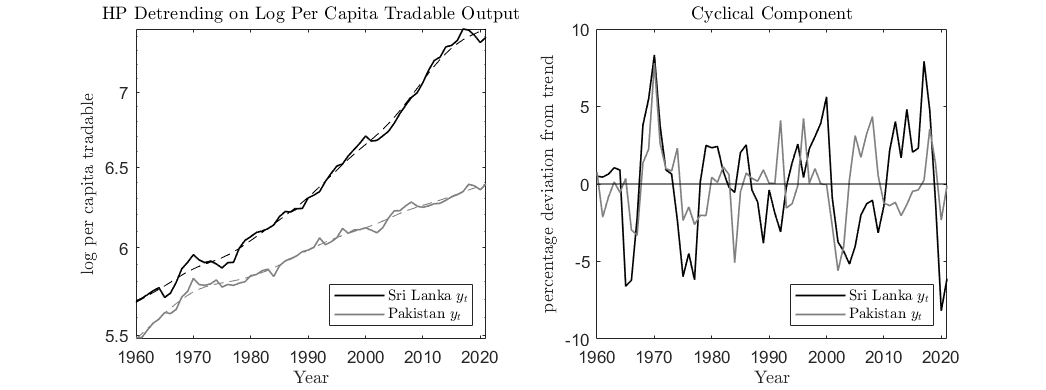
\includegraphics[height = 0.5\textheight]{fig/decompose_trad_hp.png}
        \framebreak

        Sri Lanka\\
        \begin{tabular}[pos]{rrrr}
        Filtering &
        $\rho$ &
        $\sigma$ &
        \begin{tabular}[c]{@{}r@{}}Unconditional \\ std\end{tabular} \\
        \midrule
        HP                   & 0.9114   & 0.0180   & 4.37\% \\
        Log-Q                & 0.9325   & 0.0266   & 7.38\%  \\
        \bottomrule
        \end{tabular}
        \\[2em]
        Pakistan\\
        \begin{tabular}[pos]{rrrr}
        Filtering &
        $\rho$ &
        $\sigma$ &
        \begin{tabular}[c]{@{}r@{}}Unconditional \\ std\end{tabular} \\
        \midrule
        HP                  & 0.8518   & 0.0116  & 2.21\%  \\
        Log-Q               & 0.9239   & 0.0174  & 4.55\%  \\  \bottomrule
        \bottomrule
        \end{tabular}

    \end{frame}


    \begin{frame}
        \frametitle{Sri Lanka}
        \begin{itemize}
            \item Time span: Before 2008, China started to provide large loans
            \item Reenty to international credit market: Since no default in the past, follow literature and choose 0.0385
            \item Debt-to-tradable-GDP ratio
            \begin{itemize}
                \item Data: 118\% average annnual
                \item Haircut: use average sovereign haircut = 37\% according to \citet{Cruces-Trebesch-13}
                \item times four to make it quarter
                \item $118\% \times 0.37 \times 4 = 175\%$
            \end{itemize}
            \item Default frequency per century: There is ambiguity in counting default events. Therefore, set as 2.6 following literature
            \item Output loss: Set as 7\% following literature
        \end{itemize}

    \end{frame}

    \begin{frame}
        \centering
        \begin{tabular}{@{}lll@{}}
        % \begin{tabular}{@{}lp{0.6\textwidth}lp{0.3\textwidth}@{}}
        \toprule
        Parameter  & Value  & Source                                                                         \\ 
        \midrule
        $\rho$     & 0.9114  & Estimation of AR(1) on GDP\\
        $\sigma_u$ & 0.0180 & Estimation of AR(1) on GDP \\
        $r^*$      & 0.01 & U.S. 3-month treasury bill rate \\
        $\theta$   & 0.0385 & \citet*{Chatterjee-12}                                              \\
        $\alpha$   & 0.65   & \citet{Jegajeevan-Sri-Lanka-DSGE}                                                       \\
        $a$        & 0.35   & Share of tradable goods in GPD                  \\
        $\xi$      & 0.5   & \citet{Na-18}                             \\
        $\sigma$   & 2   & $1 / \xi$                                                                      \\
        $\gamma$   & 1.109   & \citet*{wage-rigidity-data}                  \\
        $\beta$    & 0.6919  &  Estimated                                                                              \\
        $\delta_1$ &  -0.4391 &   Estimated                                                                             \\
        $\delta_2$ &  0.5530   &               Estimated                                                                 \\
        $\bar{h}$  & 1      & Normalized to 1\\
        \bottomrule
        \end{tabular}%

    \end{frame}

    \begin{frame}
        \frametitle{Pakistan}
        \begin{itemize}
            \item Time span: Before 2013, China started to provide large loans
            \item reentry to international credit market: 1999 default $\rightarrow$ 2004 gain possitive flow $\rightarrow$ 6 years, or 24 quarters
            \item Debt-to-tradable-GDP ratio
            \begin{itemize}
                \item Data: 69\% average annnual
                \item Haircut: use average sovereign haircut = 37\% according to \citet{Cruces-Trebesch-13}
                \item times four to make it quarter
                \item $69\% \times 0.37 \times 4 = 102\%$
                \item (Typo in the thesis)
            \end{itemize}
            \item Default frequency per century: There is ambiguity in counting default events. Therefore, set as 2.6 following literature
            \item Output loss: Set as 7\% following literature
        \end{itemize}

    \end{frame}

    \begin{frame}
        \centering
        \begin{tabular}{@{}lll@{}}
        % \begin{tabular}{@{}lp{0.6\textwidth}lp{0.3\textwidth}@{}}
        \toprule
        Parameter  & Value  & Source                                                                         \\ 
        \midrule

        $\rho$     & 0.8518 & Estimation of AR(1) on GDP\\
        $\sigma_u$ & 0.0116 & Estimation of AR(1) on GDP\\
        $r^*$      & 0.01 & 3 month treasury bill rate \\
        $\theta$   & 0.0417 & \citet*{trebesch-2011-sovereign}                                              \\
        $\alpha$   & 0.4   & \citet{Pakistan-DSGE-calibration}                                                       \\
        $a$        & 0.33   &Share of tradable goods in GDP                    \\
        $\xi$      & 0.5   & \citet{Na-18}                              \\
        $\sigma$   & 2   & $1 / \xi$                                                                      \\
        $\gamma$   & 1.048   & \citet*{wage-rigidity-data}                  \\
        $\beta$    & 0.6252  &  Estimated \\
        $\delta_1$ &  -0.5148 &   Estimated  \\
        $\delta_2$ &  0.5789   &     Estimated   \\
        $\bar{h}$  & 1      & Normalized to 1\\
        \bottomrule
        \end{tabular}%
    \end{frame}

    \section{Result}

    \begin{frame}[label = {sri_ds}]
        \frametitle{Sri Lanka Default Set}
        \centering
        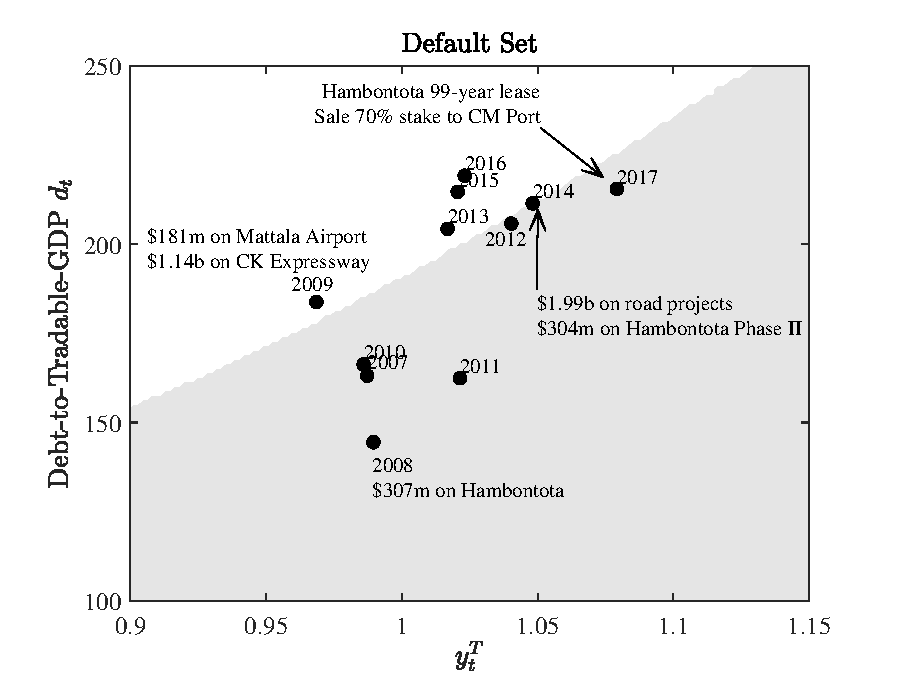
\includegraphics[width = 0.8 \textwidth]{fig/default_set_sri_trad_hp_with_china.eps}\\
    \end{frame}

    \begin{frame}[label = {pak_ds}]
        \frametitle{Pakistan Default Set}
        \centering
        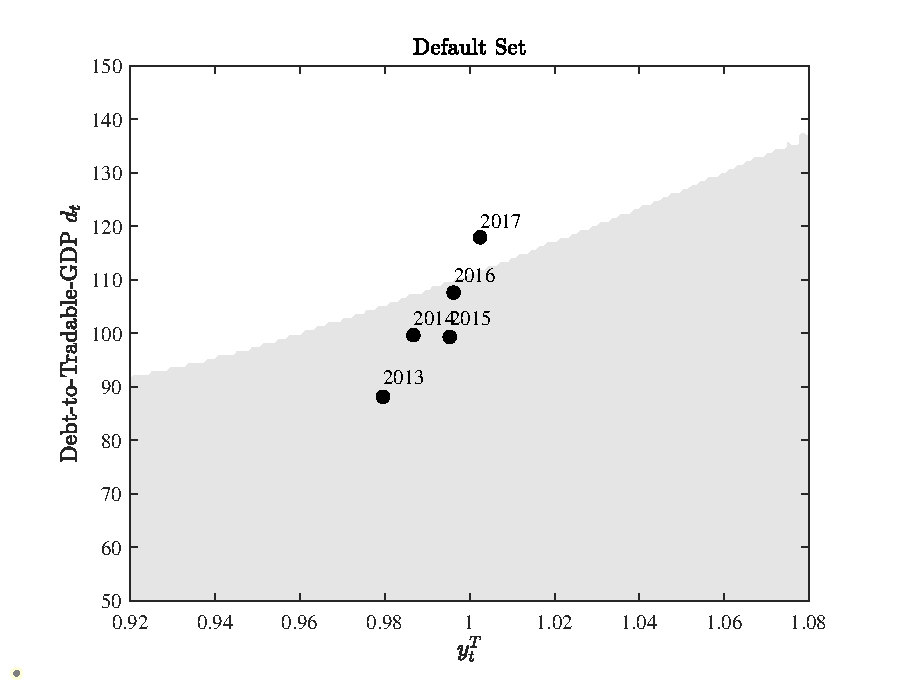
\includegraphics[width = 0.8 \textwidth]{fig/default_set_pak_trad_hp_with_china.eps}\\
    \end{frame}

    \begin{frame}
        \frametitle{Removing China's Debt}
        \centering
        \only<1-2>{Sri Lanka\\}
        \only<3-4>{pakistan\\}
        \includegraphics<1>[width = 0.8 \textwidth]{fig/sri_with_china.png}%
        \includegraphics<2>[width = 0.8 \textwidth]{fig/sri_x_china.png}%
        \includegraphics<3>[width = 0.8 \textwidth]{fig/pak_with_china.png}%
        \includegraphics<4>[width = 0.8 \textwidth]{fig/pak_x_china.png}%
    \end{frame}

    \begin{frame}
        \frametitle{Problems with Removing China's Debt}

        \begin{itemize}
            \item Debt is endogenous in the model --- Might borrow from other countries
            \begin{itemize}
                \item Hambantota Port is originally the former President's idea
                \item Pakistan is under severe power shortage, might borrow money for infrastructure constructions
            \end{itemize}
            \item GDP might be lower --- BRI investment might have cause the counties' GDP to grow
            \begin{itemize}
                \item BRI investment may increase labor demand on industrial sectors
            \end{itemize}
            \item Counterfactual analysis must account for the two factor.
        \end{itemize}
    
        
    
    \end{frame}

    \begin{frame}
        \frametitle{Robustness Check}
    
        \begin{itemize}
            \item HP-filter or Log-Quadratic?
        \end{itemize}

        \begin{tabular}{@{}rrrrrrr@{}}
        \toprule
        \multicolumn{1}{c}{} & \multicolumn{3}{c}{Sri Lanka} & \multicolumn{3}{c}{Pakistan} \\ \cmidrule(l){2-7}
        Filtering &
        $\beta$ &
        $\delta_1$ &
        $\delta_2$ &
        $\beta$ &
        $\delta_1$ &
        $\delta_2$\\
        \midrule
        HP &    0.6919 &  -0.4391  &  0.5530 &  0.6252 &  -0.5148  &   0.5789 \\
        Log-Q &0.6320  & -0.2878  &  0.4248  &   0.8627   & -0.4167    & 0.4973\\  \midrule
        &
        $d/y^T$ &
        freq &
        $L$ &
        $d/y^T$ &
        freq &
        $L$ \\
        \midrule
        \textbf{\emph{Target}} &
    \emph{ 1.75} &\emph{ 2.6} &\emph{ 0.07} &\emph{ 1.02} &\emph{ 2.6} &\emph{ 0.07} \\
        HP &  1.73 &	1.26 & 0.102 & 1.02 & 1.26 & 0.057\\
        Log-Q & 1.70 & 1.8 & 0.122 & 1.00 & 1.06 & 0.067\\
        \bottomrule

        \end{tabular}
    \end{frame}

    \begin{frame}
        \frametitle{Sri Lanka -- Log-quadratic}
        \centering
        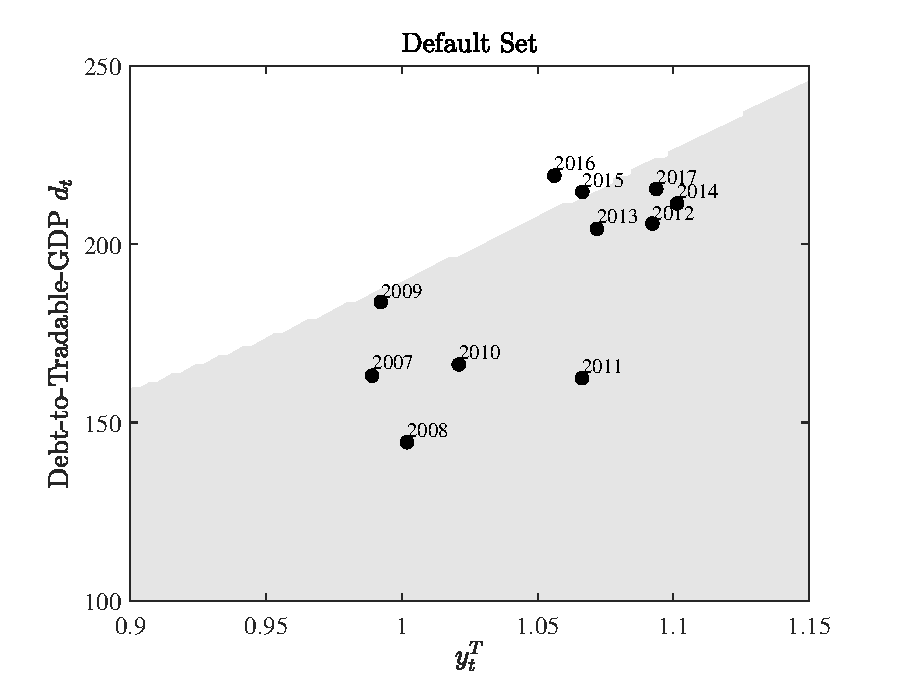
\includegraphics[width = 0.8 \textwidth]{fig/default_set_sri_trad_logq_with_china.eps}
    
    \end{frame}

    \begin{frame}
        \frametitle{Pakistan -- Log-quadratic}
        \centering
        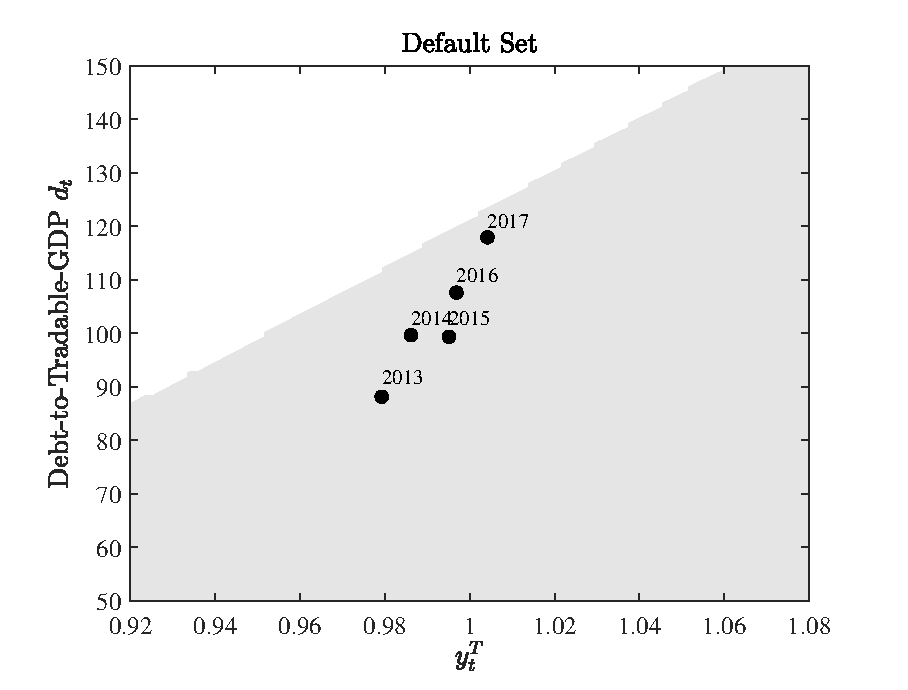
\includegraphics[width = 0.8 \textwidth]{fig/default_set_pak_trad_logq_with_china.eps}
    
    \end{frame}
    \appendix
    \begin{frame}[allowframebreaks]
            \frametitle{References}
            \bibliographystyle{econ}
            \bibliography{bib/ref}
    \end{frame}
\end{document}